\documentclass[10pt,a4paper]{article}
\usepackage[margin=2.2cm]{geometry}
\usepackage{fontspec}
\usepackage{kotex}
\setmainfont{Apple SD Gothic Neo}
\setsansfont{Apple SD Gothic Neo}
\usepackage{amsmath,amssymb}
\usepackage{graphicx}
\usepackage{booktabs}
\usepackage{caption}
\usepackage[dvipsnames]{xcolor}
\usepackage[colorlinks=true,linkcolor=MidnightBlue,citecolor=MidnightBlue,
            urlcolor=MidnightBlue]{hyperref}
\usepackage{titlesec}
\titleformat{\section}{\large\bfseries}{\thesection}{0.6em}{}
\titleformat{\subsection}{\normalsize\bfseries}{\thesubsection}{0.5em}{}
\captionsetup{font=small,labelfont=bf}
\setlength{\parskip}{0.35em}
\setlength{\parindent}{0pt}

\usepackage{mdframed}
\newmdenv[linewidth=0.4pt,linecolor=gray!60,backgroundcolor=gray!5,
          innertopmargin=6pt,innerbottommargin=6pt,skipabove=8pt,skipbelow=8pt]{claimbox}
\newcommand{\claim}[2]{\begin{claimbox}\textbf{주장.} #1\par\smallskip
  \textcolor{gray!70}{\textbf{반증 조건.} #2}\end{claimbox}}

\title{\bfseries $2{,}028$행이 필요하다\\[2pt]
\large 판정력을 먼저 재니 $62$행으로는 방문객 $10\%$ 차를 못 가른다 --- 그리고 같은
부트 분포를 두 자로 읽으면 답이 $44{,}000$배 달랐다}
\author{월드모델 실험실 · 노트 770 · 771 (노트 688 을 잇는다)}
\date{2026-08-07}
\begin{document}\maketitle

\section{한 줄}

논문 $151$ 이 T2 의 마지막 물음을 \textbf{법칙 물음}으로 좁혔다 --- 노트 $688$ 이
사전등록한 \textbf{$L(g, \text{event})$ 동네 고정 회귀}. 그 노트는 사각에
\emph{``라벨이 얇다 --- 행수를 먼저 찍고 그 수로 판정력을 적는다''}를 적어 뒀다.

\textbf{행수를 찍었다: $380 \to 179 \to 66 \to \mathbf{62}$.} 판정력을 재니
\textbf{MDE가 실무 문턱의 $5.7$배}다 --- \textbf{방문객 $10\%$ 차를 못 가른다.}
\textbf{$2{,}028$행이 필요하고 지금 $62$행이다.}

그리고 \textbf{같은 부트 분포를 SD로 읽으면 필요 행수가 $8{,}900$만, IQR로 읽으면
$2{,}028$} 이었다 --- \textbf{$44{,}000$배 차이}.

\section{판정력을 먼저 재는 것이 이번 방법이다}

논문 $151$ 의 교훈이 \emph{``자를 먼저 정한다''}였다. \textbf{그 다음 층이 이것이다}
--- 자를 정했는데 \textbf{그 자로 이 표본에서 아무것도 못 잰다면 그것이 결론이다.}

\claim{\textbf{판정력이 없으면 ``효과 없음''이 아니라 ``모른다''로 적는다.} 노트
$133$(\emph{``첫 양성을 그냥 채택하지 않는다''})의 짝이다 --- \textbf{첫 음성도, 첫
부호도 판정력 없이 읽지 않는다.}}
{판정력을 재는 것 자체가 회귀를 돌리는 것과 비슷한 비용이면 그냥 돌리는 게 낫다.
\textbf{여기서는 그렇지 않았다} --- MDE를 내려면 어차피 설계행렬과 부트가 필요하고,
그러면 계수도 같이 나온다. \textbf{즉 이 규율의 값은 계산을 아끼는 것이 아니라
\emph{결론을 아끼는} 것이다.}}

\subsection*{자료가 줄어드는 사다리}

\begin{center}
\begin{tabular}{lrl}
\toprule
& 행 & \\
\midrule
팝업 레코드 & $380$ & \\
$+$ 시군구 있음 & $179$ & \\
$+$ \textbf{방문객 라벨} & $\mathbf{66}$ & 노트 $688$ 은 $99$건으로 봤다 \\
$+$ 장 창($30$일) & $62$ & \\
$+$ 동네 고정(같은 구 $2$건 이상) & $\mathbf{62}$ & 시군구 $10$개 \\
\bottomrule
\end{tabular}
\end{center}

노트 $688$ 이 본 \emph{``동네 고정 · 시기 다름: $19$시군구 $243$행''}은 \textbf{라벨
없는 것까지 센 값}이었다.

\textbf{시군구는 손으로 표를 쓰지 않았다} --- 레코드의 \texttt{district} 가 정규화돼
있지 않지만(`성동구' · `성수' · `성동구 성수동'이 따로) \textbf{기존 해석기}
(\texttt{sgg\_index} · \texttt{hood\_sgg} · \texttt{city\_sgg})가 접었다. 노트 $661
\cdot 662$ 가 시장팝업에서 쓴 길이다.

\begin{figure}[t]\centering
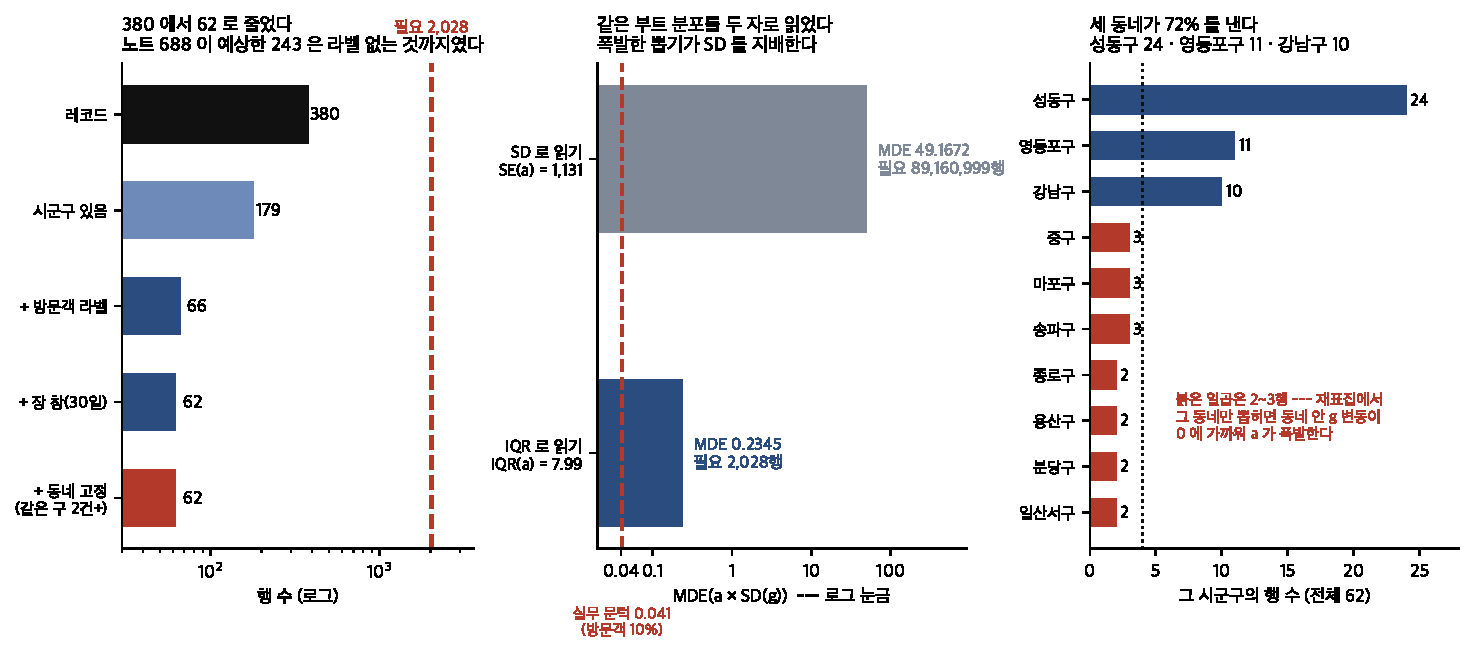
\includegraphics[width=0.99\textwidth]{figs/twothousand.pdf}
\caption{왼쪽: \textbf{$380$에서 $62$로 줄었다.} 가운데: \textbf{같은 부트 분포를 두
자로 읽으면 필요 행수가 $44{,}000$배 달라진다.} 오른쪽: \textbf{세 동네가 $72\%$를
낸다} --- 나머지 일곱이 $2{\sim}3$행이고 그것이 폭발의 원인이다.}
\end{figure}

\section{사전등록을 두 번 고쳤다}

\textbf{유효한 추정치를 보기 전에 고쳤다} --- 첫 실행은 overflow로 무효였다.

\begin{center}
\begin{tabular}{ll}
\toprule
\textbf{① 단위 불일치} & 사전등록이 \emph{``MDE$(a)$를 노트 $648$의 자국 $0.0087$과
견준다''}고 적었는데 \\
& $a$ 는 \textbf{라벨 단위$/$g 단위}이고 $0.0087$ 은 \textbf{g 단위}다 --- 견줄 수 없다 \\
& $\to$ 자를 $a \times \text{SD}(g)$ 로 바꾸고 실무 문턱을 \textbf{방문객 $10\%$
$= 0.041$ log10} 으로 못박았다 \\
\midrule
\textbf{② 명세 축소} & 사전등록 명세(시군구 FE $+$ \textbf{월 더미} $+$ prior $+$ $g$
$+$ $g{\times}$규모)는 \\
& $62$행에 모수 $24$다. 계급은 찼지만($24/24$) \textbf{클러스터 부트가 폭발한다}
(SE $187$) \\
& $\to$ 월 더미를 뺀 축소 명세(모수 $13$)로 판정하고 갑은 숫자로 남겼다 \\
\bottomrule
\end{tabular}
\end{center}

\claim{\textbf{단위를 안 보고 문턱을 적으면 그 문턱은 자가 아니다.} 규약 $18$(가드를
인용할 때 시험대를 적는다)과 규약 $13$(문턱에 $\sigma$ 를 적는다)의 세 번째 층이다 ---
\textbf{문턱에는 시험대와 $\sigma$ 와 \emph{단위}가 다 필요하다.}}
{단위를 미리 못 본 것은 회귀를 짜기 전이라 $a$ 의 단위가 확정되지 않았기 때문이다.
\textbf{그렇다면 사전등록에 ``자의 단위는 명세를 짠 뒤에 확정한다''를 적어 두는 것이
정직하다} --- 그러면 나중 정정이 규칙 변경이 아니라 예정된 절차가 된다.}

\section{같은 분포를 두 자로 읽었다}

\begin{center}
\begin{tabular}{lrrl}
\toprule
& MDE$(a \times \text{SD}(g))$ & 필요 행수 & \\
\midrule
\textbf{SD}로 읽기 (SE$(a) = 1{,}131$) & $49.17$ & $\mathbf{89{,}160{,}999}$ & 쓸 수 없다 \\
\textbf{IQR}로 읽기 (IQR$(a) = 7.99$) & $\mathbf{0.2345}$ & $\mathbf{2{,}028}$ & 쓸 수 있다 \\
\midrule
실무 문턱 (방문객 $10\%$) & $0.041$ & --- & \\
\bottomrule
\end{tabular}
\end{center}

\textbf{원인이 클러스터 크기다.} $62$행이 시군구 $10$개에 \textbf{성동구 $24$ ·
영등포구 $11$ · 강남구 $10$} 으로 몰려 있고 \textbf{나머지 일곱이 $2{\sim}3$행}이다.
재표집에서 작은 동네만 뽑히면 \textbf{동네 안 $g$ 변동이 $0$ 에 가까워 $a$ 가
폭발}한다($g$ 동네안 SD가 전체로도 $0.0217$ 뿐이다).

\claim{\textbf{클러스터 부트스트랩은 SD가 아니라 IQR로 읽는다.} $\text{MDE} = 1.35
\times \text{IQR}$ 로 환산한다. 규약 $25$(자를 최댓값으로 만들지 않는다)의 \textbf{세
번째 층}이다 --- 최댓값 · 최댓값-지배 SD · 폭발 뽑기.}
{IQR도 임의 선택이다 --- $5{\sim}95\%$ 로 읽으면 또 다른 값이 나온다($-385 \sim
+2546$). \textbf{그러면 어느 자가 옳은가는 ``무엇을 물었나''가 정한다}: ``이 표본으로
전형적인 경우 무엇을 가릴 수 있나''를 물었으므로 \textbf{중앙 절반}이 맞는 자다.
\textbf{그 선택을 적어 두는 것이 이 논문의 의무이고, 다른 자로 읽으면 결론이 바뀔 수
있다는 뜻이다} --- 다만 어느 자로 읽어도 $62$행이 $0.041$ 을 가르지는 못한다.}

\section{그래서 무엇을 말할 수 있나}

\begin{center}
\begin{tabular}{ll}
\toprule
\textbf{말할 수 있는 것} & $62$행 · 시군구 $10$개로는 \textbf{방문객 $10\%$ 차를 못
가른다}(MDE가 $5.7$배) \\
& \textbf{$2{,}028$행이 필요하다}(현재의 $33$배) \\
\midrule
\textbf{말할 수 없는 것} & $a$ 의 부호. 점추정 $a \times \text{SD}(g) = -0.0454$ 이고 \\
& 노트 $688$의 규칙 ④(\emph{``뜨거운 시기에 여는 팝업이 더 나쁘다 --- 경쟁 밀도''})를
가리키지만 \\
& \textbf{MDE가 그 $5.2$배다} \\
\bottomrule
\end{tabular}
\end{center}

\claim{\textbf{T2 를 쉼으로 내린다 --- 다시 열 조건을 값으로 적는다.} 이 트랙의 물음
넷이 다 끝났다: \textbf{판 통로 셋 폐쇄}(논문 $150$) · \textbf{상품 번역
실패}(논문 $151$ · $R^2$ $0.1200$ 이 전체의 $0.236\%$) · \textbf{법칙 물음 판정
불가}(여기). \textbf{조건: 시군구 고정 가능한 방문객 라벨 $2{,}028$행.}}
{$2{,}028$ 은 \textbf{현재 표본의 구조가 그대로 커진다}는 가정에서 나온 수다. 새 행이
\textbf{작은 동네에 골고루} 들어오면 클러스터 균형이 좋아져 더 적게 필요할 수 있고,
성동구에만 더 쌓이면 더 많이 필요하다. \textbf{그래서 요청은 ``$2{,}028$행''이 아니라
``$2{,}028$행 \emph{그리고} 동네가 골고루''다.}}

\subsection*{그 행수는 채굴이 아니라 생성으로 와야 한다}

방문객 라벨은 이미 전수로 캤다 --- 노트 $635$가 이미지 PDF $77$건을 전수 판독하고
\emph{``조직이 방문객을 안 센다''}를 확정했다. \textbf{그러므로 $62 \to 2{,}028$ 은
채굴로 안 온다.} 노트 $673$ 이 본 것이 길이다 --- BQ \texttt{core.engagement}
$578$건 대 우리 레코드 $380$건, \textbf{레코드가 없는 engagement}. 그것은
\textbf{T7(수집)의 물음}이다.

\end{document}
